\begin{figure*}[t]
    \centering
    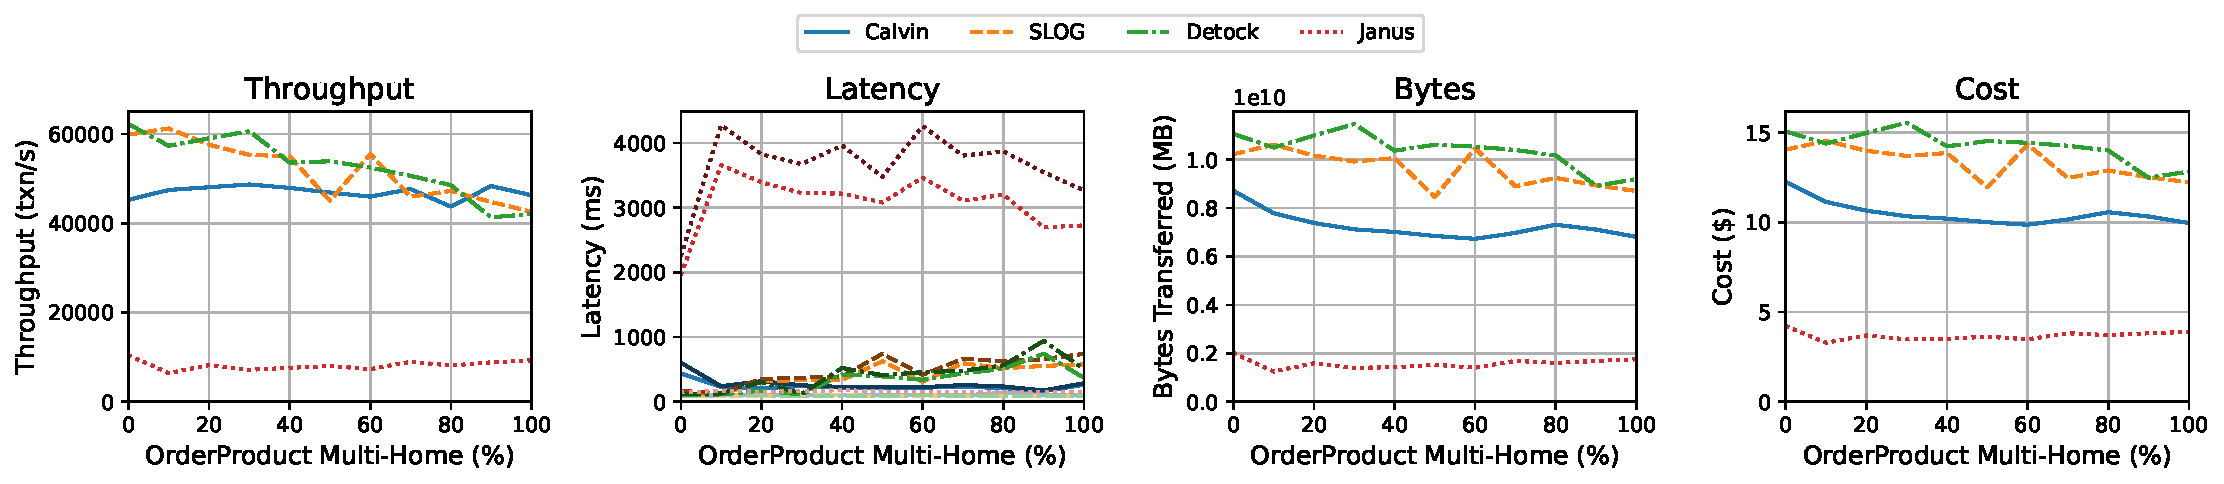
\includegraphics[width=1\textwidth]{figures/Baseline.pdf}
    \caption{Results of the Baseline Scenario.}
    \label{fig: baseline-scenario}
\end{figure*}

\begin{figure*}[t]
    \centering
    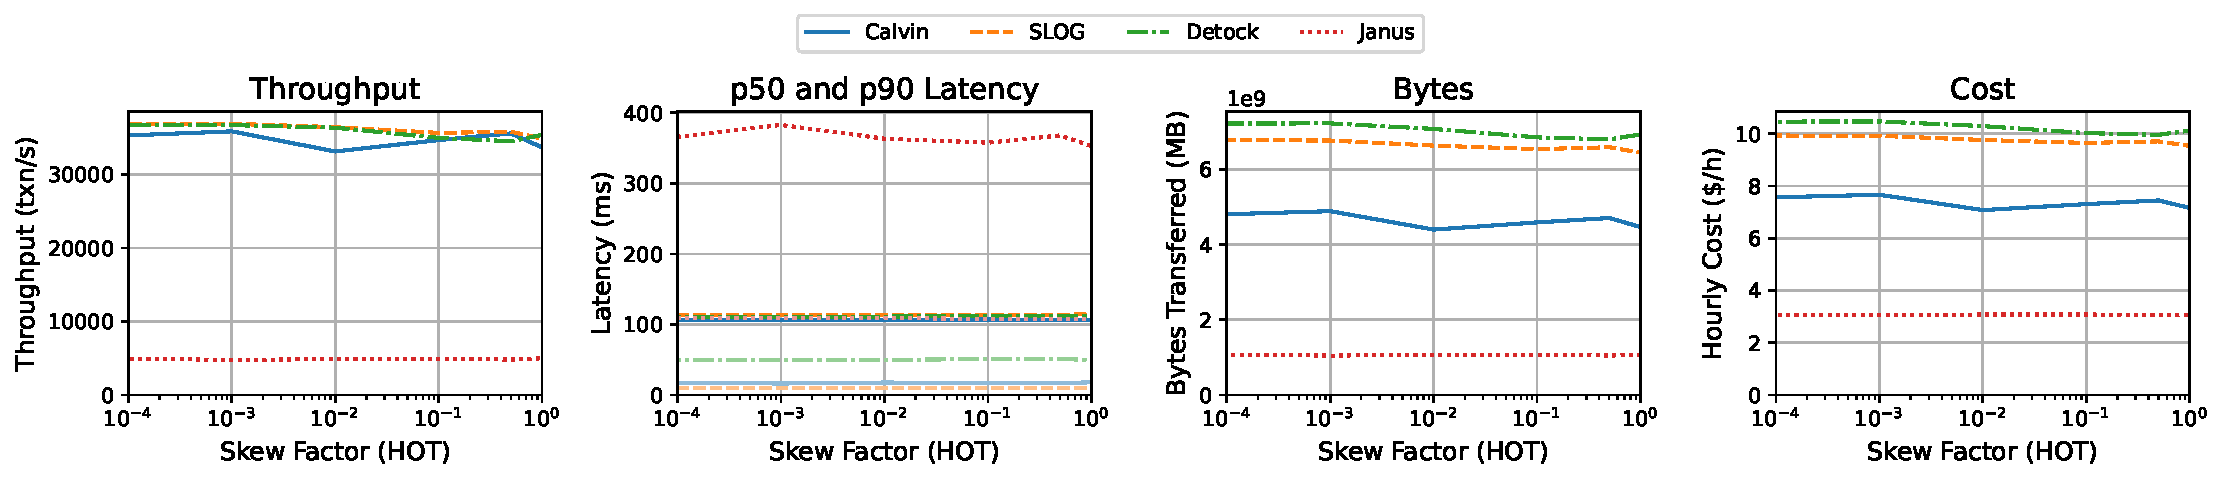
\includegraphics[width=1\textwidth]{figures/Skew.pdf}
    \caption{Results of the Skew Access Scenario.}
    \label{fig: skew-access-scenario}
\end{figure*}

\section{Experimental Setup and Results}
\label{sec: experimental-setup-and-results}
This section outlines our experimental methodology and key findings. Section~\ref{subsec: deployment-and-metrics-collection} describes our deployment setup and the methodology used for performance measurement, and Section~\ref{subsec: evaluation-scenarios-and-results} presents the results obtained under a range of different experimental scenarios.

\subsection{Deployment and Metrics Collection}
\label{subsec: deployment-and-metrics-collection}
We conducted all experiments on a dedicated 4-node high-performance cluster located in our university. Each node is equipped with dual AMD EPYC 7H12 processors, 256 hardware threads, and 503 GiB of RAM. The nodes are interconnected via 10 Gigabit Ethernet.

In our experiments, we simulated a two-region deployment by using all four physical nodes and injecting artificial network delay between them. Both clients and servers are deployed as Docker containers to ensure a clean and reproducible environment. Figure~\ref{fig: overall-architecture} illustrates the setup. The data is divided into two partitions, and each logical region consists of two server containers that hold a complete copy of both partitions. The cluster delivers a natural intra-region round-trip time (RTT) of roughly 0.15 ms, and we set the inter-region RTT to 100 ms (Table~\ref{tab: rtt-machines}).

\begin{table}[htbp]
  \centering
  \begin{tabular*}{\linewidth}{@{\extracolsep{\fill}} l r r r r}
    \toprule
               & \textbf{A-P1} & \textbf{A-P2} & \textbf{B-P1} & \textbf{B-P2} \\ \midrule
    \textbf{A-P1} & —      & 0.15 ms & 100 ms & 100 ms \\
    \textbf{A-P2} & —      & —      & 100 ms & 100 ms \\
    \textbf{B-P1} & —      & —      & —      & 0.15 ms \\
    \textbf{B-P2} & —      & —      & —      & —      \\ 
    \bottomrule
  \end{tabular*}
  \caption{Round-trip times between all unordered pairs of machines. We uniquely identify the machines with the label \textit{Region-Partition} (e.g., \textit{A-P1} is the partition 1 within the region A).}
  \label{tab: rtt-machines}
\end{table}

Unless stated otherwise, the clients are uniformly distributed across the two regions. To avoid overwhelming or underdriving the systems, we first explore the effects of the number of clients using the scalability test from Section~\ref{subsubsec: scalability-scenario}. We identify for each system the point where additional clients would no longer increase the throughput, and use that client count in all remaining scenarios.

For performance evaluation, each client container collects local metrics during execution, which are then aggregated by a centralized admin. The metrics we focus on are throughput, latency, abort rates, and bytes transferred, and we also estimate the operational cost. Throughput, latency, and abort rates are measured directly by the application logic, while the number of transferred bytes is collected using system-level network monitoring tools. Additionally, we provide a simplistic estimation of the operational cost by monitoring the resource utilization within the server containers and tracking the overall network usage. The formula we use for the hourly cost is $C = N_{\text{machine}} * P_{\text{machine}} + V_{\text{traffic}} * P_{\text{traffic}}$, where $N_{\text{machine}}$ is the number of server containers, $P_{\text{machine}}$ is the on-demand hourly price for the each used machine, $V_{\text{traffic}}$ is the cross-region traffic volume, and $P_{\text{traffic}}$ is the data transfer price.

\subsection{Evaluation Scenarios and Results}
\label{subsec: evaluation-scenarios-and-results}
We now describe the experimental scenarios used in our evaluation. We designed these scenarios to systematically observe the impact of different system configurations on the transactional performance of the database systems. Each scenario is strongly connected with the tunable parameters shown in Figure~\ref{fig: overall-architecture}, which control the network conditions, the clients' placement, and the transactional load.

\subsubsection{Baseline Scenario}
\label{subsubsec: baseline-scenario}
In the baseline scenario, we aim to understand how each concurrency control protocol performs under standard conditions in the two-region deployment with no artificial skew, packet loss, or extra delay besides the default link latencies shown in Table~\ref{tab: rtt-machines}. Specifically, we vary only the fraction of \textit{multi-home transactions} among the \textit{OrderProduct} type while keeping the proportion of multi-partition transactions constant at 50\%. This scenario allows us to isolate the cost of coordination across different geographical regions. Figure~\ref{fig: baseline-scenario} shows the metrics collected for each protocol: the throughput, the median latency ($p50$), along with the $90^{th}$-percentile latency ($p90$), the bytes transferred, and the hourly operational cost.

Among all systems, Janus has the lowest throughput and the highest latencies. This is primarily because Janus does not have the notion of multi-home transactions, and routes every commit through its integrated consensus path, which requires cross-region coordination even for transactions that could be executed locally. As a consequence, the throughput stays constant, and even the single-region transactions need at least one WAN round-trip, which is visible in the plot as the $p50$ latency sits near the inter-region RTT ($\approx$100 ms). In case of conflicts, Janus needs an additional wide-area round-trip, so $p90$ latency exceeds 200 ms, and even slightly increases with larger MH fractions, since this inherently increases the contention, as the regions will contend for the same products.

Calvin also does not have the notion of multi-home transactions, and thus, the throughput stays almost constant. It performs worse than SLOG and Detock when the proportion of multi-home transactions is low, but it overtakes them as the proportion exceeds roughly $60\%$. This is because Calvin relies on a deterministic global sequencer that orders all transactions. When most transactions are local, Calvin's overhead for global ordering becomes unnecessary and costly, but as the proportion of multi-home transactions increases, Calvin's global sequencer can coordinate them efficiently and get a better performance than SLOG and Detock, which incur a significant cost of handling multi-home transactions.

\subsubsection{Skewed Access Scenario}
\label{subsubsec: skew-access-scenario}
In the skewed access scenario, we study how each protocol handles the contention caused by an uneven access pattern. We fix the workload composition so that half of the \textit{OrderProduct} transactions are multi-home, and similarly, half of them are multi-partition. To introduce skew, we use the NURand distribution to define so-called \textit{hot records} that will be accessed more often depending on the \textit{skew factor} \cite{council2010tpc}.

As shown in Figure~\ref{fig: skew-access-scenario}, the curves remain nearly flat for all four systems across the entire range of skew factors. For the deterministic designs (Calvin, SLOG, Detock), this is expected since each replica already knows the global order before the execution begins, so a hot key cannot block related transactions. The skew also has little effect on Janus, showing that the system's bottleneck is given by the WAN round-trip.

\begin{figure*}[ht]
    \centering
    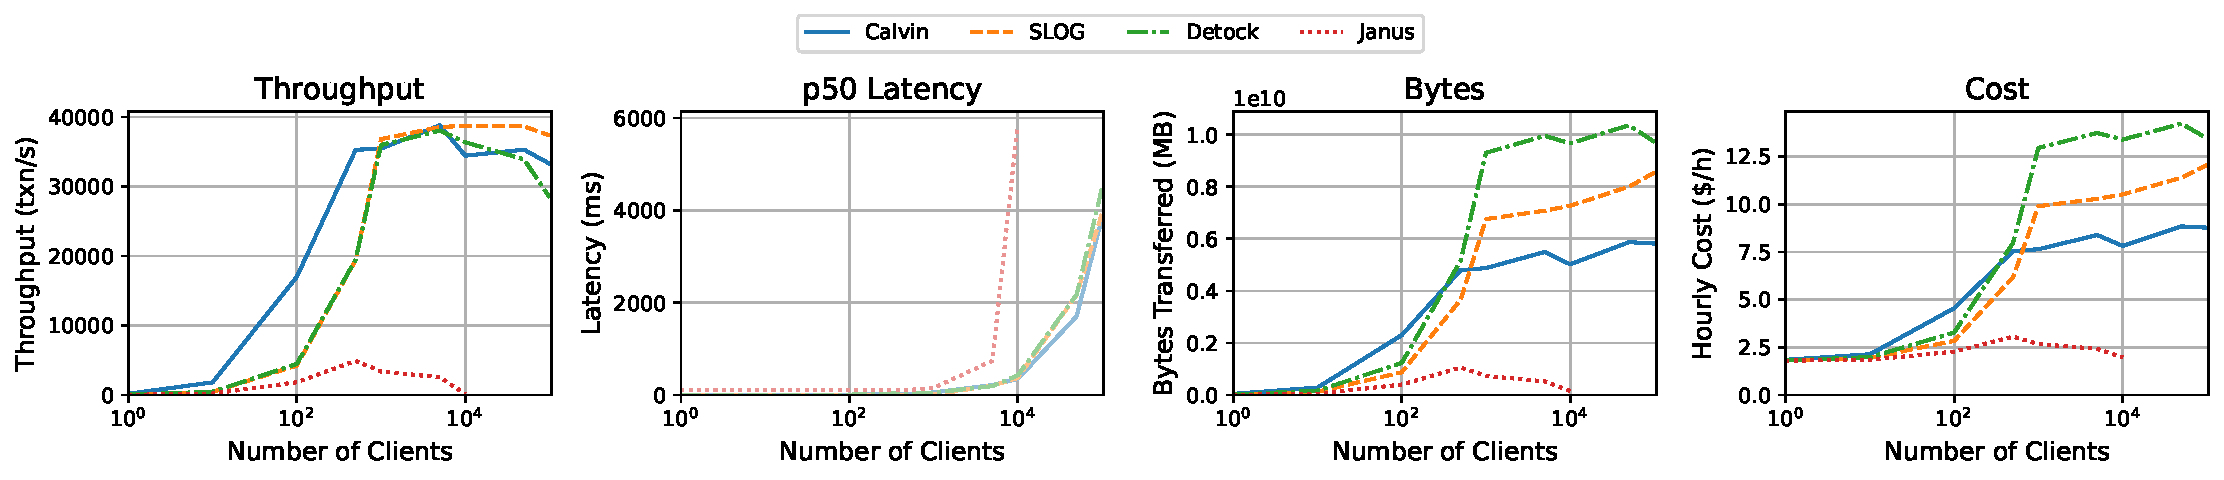
\includegraphics[width=1\textwidth]{figures/Scalability.pdf}
    \caption{Results of the Scalability Scenario.}
    \label{fig: scalability-access-scenario}
\end{figure*}

Figure~\ref{fig: abort-rates} reveals the hidden cost of the skew. The protocols themselves don't abort transactions, since Calvin, SLOG, and Detock commit every transaction in the predetermined order, and Janus commits according to the serialization graph. Therefore, all aborts we observe come from the way we execute the dependent transaction \textit{OrderProduct}. We split it into a read-only phase that retrieves the parts currently associated with the given product, and a write phase that performs the updates. If any of those parts change between those two phases, the server aborts the second phase and signals the client to retry the whole transaction starting from the first phase. The presence of hot records raises the chance that the second phase's validation fails, which explains why abort rates increase with the skew for all systems. However, the increase is small, peaking at only $2.5\%$ among all systems, and leaving throughput and latency practically unchanged.

\begin{figure}[ht]
  \centering
  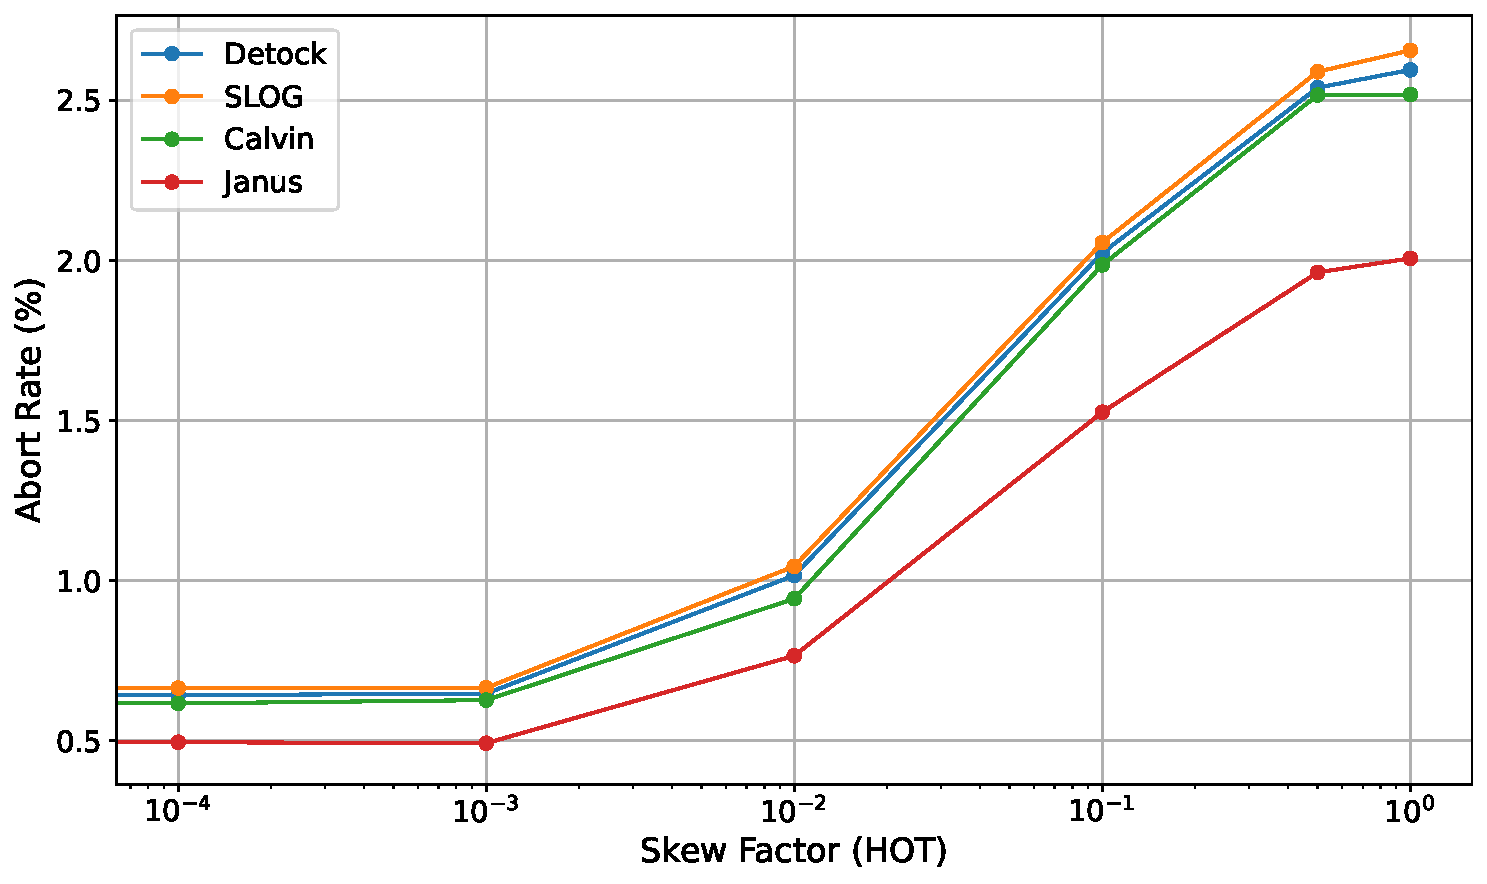
\includegraphics[width=\columnwidth]{figures/Abort Rates.pdf}
  \caption{Abort Rates in the Skew Access Scenario.}
  \label{fig: abort-rates}
\end{figure}

\subsubsection{Sunflower Topology Scenario}
\label{subsubsec: sunflower-topology-scenario}
The sunflower experiment analyzes how the protocols react when one region turns into a central hub. This is a common occurrence in the real world, where deployments rarely receive perfectly balanced traffic. A viral event, a seasonal sale, or an outage in a neighboring zone can redirect requests into one data centre while the others stay idle. To reproduce this, we perform a 100-second run, where we start with balanced traffic, and then linearly increase the share of transactions whose home region is \textit{Region A} (or, for multi-home transactions, include \textit{Region A} in the home set) with 10\% every 10 seconds, until it receives the entire load. Throughout the experiment, we keep the workload mix fixed at $50\%$ multi-partition and $50\%$ multi-home transactions, and leave the default RTTs unchanged, so any throughput change reflects only the growing regional imbalance.

Figure~\ref{fig: sunflower-throughput} plots the resulting throughput. At the start, when traffic is evenly split, all systems have their baseline throughput. As the bias grows, SLOG and Detock are the only ones that experience a decrease in throughput. Once more requests land in the same region, the single-home fast path overwhelms the replica while its counterpart in \textit{Region B} sits mostly idle, so the aggregate throughput drops.

In contrast, Calvin's throughput stays approximately the same. In the Detock codebase, Calvin's global sequencer uses a replication based on a primary replica by asynchronously sending every transactional input (both the single-home and multi-home transactions) to a dedicated region that broadcasts the batches in order. Since the primary replica already acts as a central point, increasing the bias doesn't have an effect on the overall throughput. Similar to the skew access scenario (\ref{subsubsec: skew-access-scenario}), Janus once again shows the lowest absolute throughput, but it is practically insensitive to the bias. Every commit must gather a WAN approval, so moving clients from \textit{Region A} to \textit{Region B} doesn't affect the throughput.

\begin{figure}[ht]
  \centering
  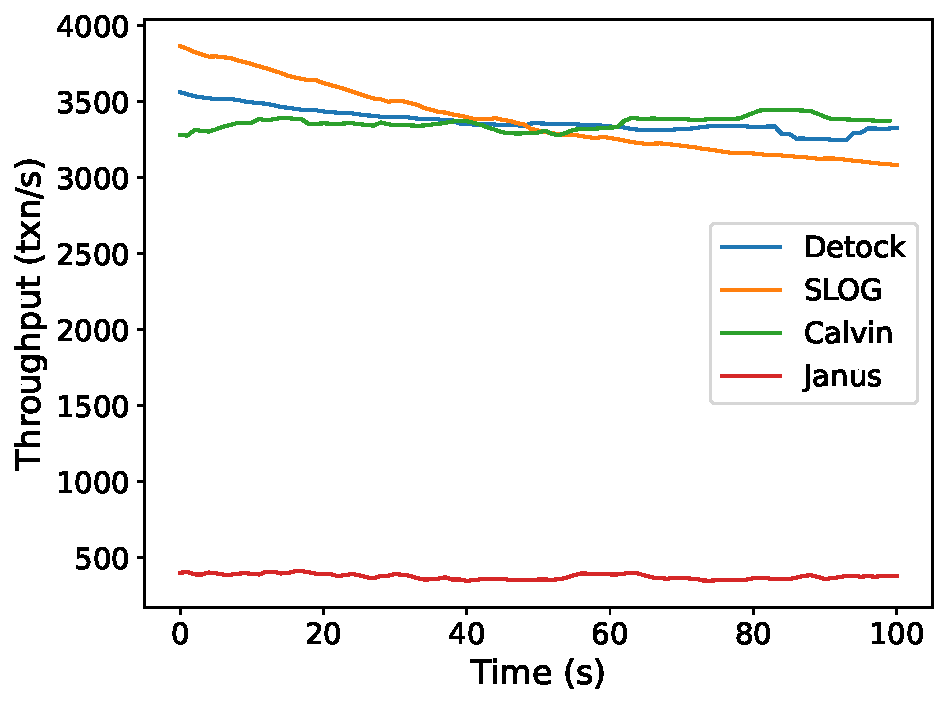
\includegraphics[width=\columnwidth]{figures/Sunflower Throughput.pdf}
  \caption{Throughput in the Sunflower Topology Scenario.}
  \label{fig: sunflower-throughput}
\end{figure}

\begin{figure*}[ht]
    \centering
    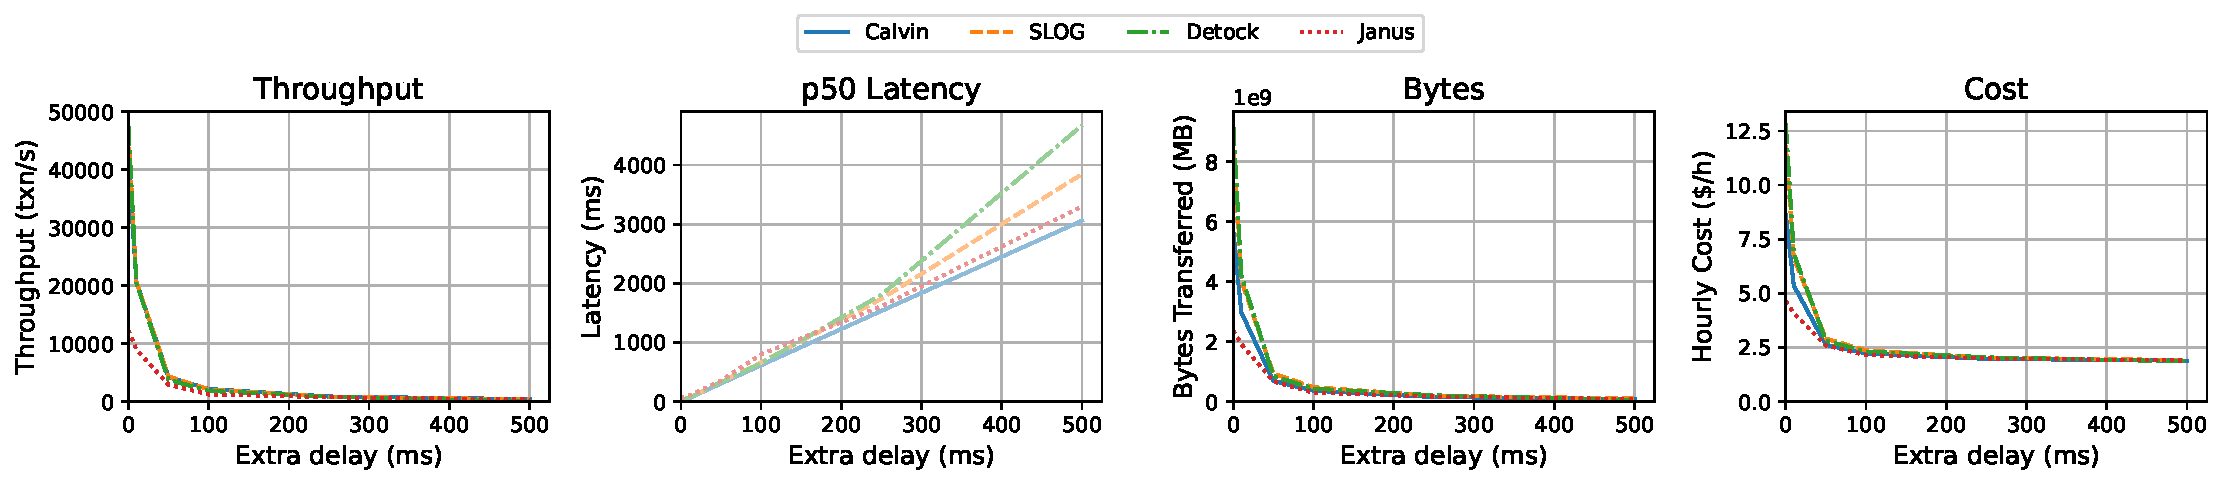
\includegraphics[width=1\textwidth]{figures/Network.pdf}
    \caption{Results of the Network Delays Scenario.}
    \label{fig: network-delays-scenario}
\end{figure*}

\begin{figure*}[ht]
    \centering
    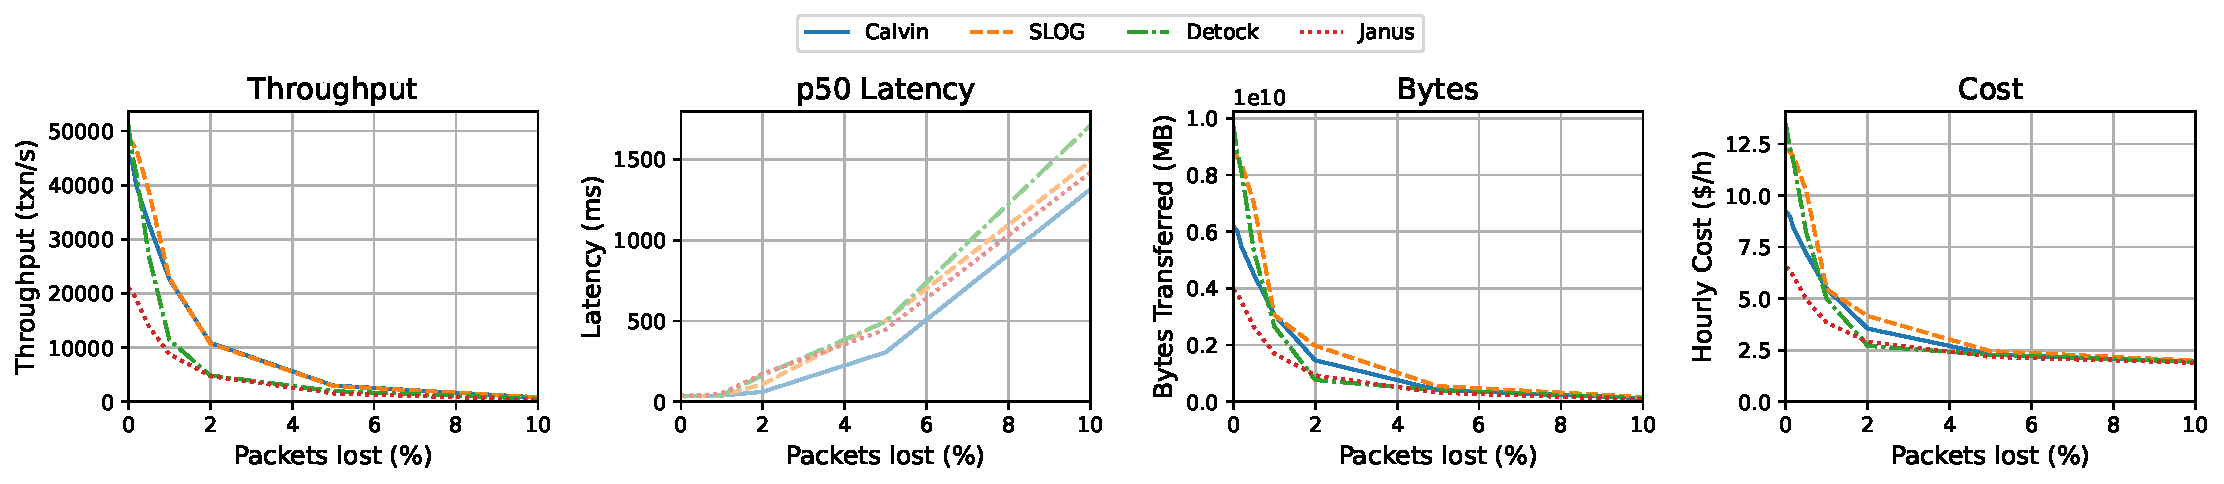
\includegraphics[width=1\textwidth]{figures/Packet Loss.pdf}
    \caption{Results of the Packet Loss Scenario.}
    \label{fig: packet-loss-scenario}
\end{figure*}

\subsubsection{Scalability Scenario}
\label{subsubsec: scalability-scenario}
The scalability scenario focuses on evaluating how each protocol performs as we increase the number of clients, while keeping the workload composition fixed at its standard configuration with $50\%$ multi-home transactions, $50\%$ multi-partition transactions, and no added skew. Figure~\ref{fig: scalability-access-scenario} shows how SLOG, Detock, and Calvin all have similar improvements in throughput as the load increases, which demonstrates that these systems have good scalability given a balanced transactional workload. Janus, on the other hand, scales to roughly 1000 clients, then its throughput collapses to 0. The likely reason is that Janus's unified consensus and replication layer has to handle more and more dependency checks in the serialization graph, which overwhelms its CPUs and network links until it can no longer make progress.

\subsubsection{Network Delays Scenario}
\label{subsubsec: network-delays-scenario}
This scenario explores how extra latency affects each system. We inject an additional delay on every cross-region link while keeping the packet loss at $0\%$ and using the standard workload mix from Section~\ref{subsubsec: scalability-scenario}. Figure~\ref{fig: network-delays-scenario} plots the results. The throughput decreases exponentially for all systems as the round-trip time grows. We note that the median latencies increase linearly with the injected delay, and Calvin's latency curve remains the lowest. This indicates that Calvin uses the smallest number of messages per transaction. Indeed, the coordinator only forwards the transactional input to the primary replica, which then broadcasts the messages in order. 

\subsubsection{Packet Loss Scenario}
\label{subsubsec: packet-loss-scenario}
In this experiment, we inject random packet loss on the WAN links, ranging from $0\%$ to $10\%$, while leaving the RTTs at their default values and the workload mix at its standard from Section~\ref{subsubsec: scalability-scenario}. Once again, the throughput falls exponentially for all systems, and Calvin proves itself the most resilient in terms of latency. This again proves Calvin's lightweight communication, which minimizes the number and size of WAN messages that can be delayed or lost.